%---------------------------------------------------------------------------------------------------
%
%	Edited by: Copyright (c) 2016 Jakub Kúdela
%   Based on: Copyright (c) 2015 Jan Küster
%
%	The MIT License (MIT)
%
%	Permission is hereby granted, free of charge, to any person obtaining a copy
%	of this software and associated documentation files (the "Software"), to deal
%	in the Software without restriction, including without limitation the rights
%	to use, copy, modify, merge, publish, distribute, sublicense, and/or sell
%	copies of the Software, and to permit persons to whom the Software is
%	furnished to do so, subject to the following conditions:
%	
%	THE SOFTWARE IS PROVIDED "AS IS", WITHOUT WARRANTY OF ANY KIND, EXPRESS OR
%	IMPLIED, INCLUDING BUT NOT LIMITED TO THE WARRANTIES OF MERCHANTABILITY,
%	FITNESS FOR A PARTICULAR PURPOSE AND NONINFRINGEMENT. IN NO EVENT SHALL THE
%	AUTHORS OR COPYRIGHT HOLDERS BE LIABLE FOR ANY CLAIM, DAMAGES OR OTHER
%	LIABILITY, WHETHER IN AN ACTION OF CONTRACT, TORT OR OTHERWISE, ARISING FROM,
%	OUT OF OR IN CONNECTION WITH THE SOFTWARE OR THE USE OR OTHER DEALINGS IN
%	THE SOFTWARE.
%
%---------------------------------------------------------------------------------------------------


%===================================================================================================
%	DOCUMENT DEFINITION
%===================================================================================================

%we use article class because we want to fully customize the page and dont use a cv template
\documentclass[10pt,a4paper]{article}	

%---------------------------------------------------------------------------------------------------
%	ENCODING
%---------------------------------------------------------------------------------------------------

%we use utf8 since we want to build from any machine
\usepackage[utf8]{inputenc}		

%---------------------------------------------------------------------------------------------------
%	LOGIC
%---------------------------------------------------------------------------------------------------

% provides \isempty test
\usepackage{xifthen}

%---------------------------------------------------------------------------------------------------
%	FONT
%---------------------------------------------------------------------------------------------------

% some tex-live fonts - choose your own

%\usepackage[defaultsans]{droidsans}
%\usepackage[default]{comfortaa}
%\usepackage{cmbright}
\usepackage[default]{raleway}
%\usepackage{fetamont}
%\usepackage[default]{gillius}
%\usepackage[light,math]{iwona}
%\usepackage[thin]{roboto}
\usepackage{hyperref}

% set font default
\renewcommand*\familydefault{\sfdefault} 	
\usepackage[T1]{fontenc}

% more font size definitions
\usepackage{moresize}		

%---------------------------------------------------------------------------------------------------
%	PAGE LAYOUT  DEFINITIONS
%---------------------------------------------------------------------------------------------------

%debug page outer frames
%\usepackage{showframe}			

%define page styles using geometry
\usepackage[a4paper]{geometry}		

% for example, change the margins to 2 inches all round
\geometry{top=1.75cm, bottom=-.6cm, left=1.5cm, right=1.5cm} 	

%use customized header
\usepackage{fancyhdr}		
\pagestyle{fancy}

%less space between header and content
\setlength{\headheight}{-5pt}		

%customize entries left, center and right
\lhead{}
\chead{\small{
  Eklavya Raman $\cdot$ 
  Student at IISER Kolkata $\cdot$ 
  Nadia, West Bengal $\cdot$ 
  \textcolor{sectcol}{\textbf{\href
  {mailto:er24ms024@iiserkol.ac.in}
  {er24ms024@iiserkol.ac.in}}} $\cdot$
  +91 9560040793
}}
\rhead{}

%indentation is zero
\setlength{\parindent}{0mm}

%---------------------------------------------------------------------------------------------------
%	TABLE /ARRAY DEFINITIONS
%--------------------------------------------------------------------------------------------------- 

%for layouting tables
\usepackage{multicol}			
\usepackage{multirow}

%extended aligning of tabular cells
\usepackage{array}
\newcolumntype{x}[1]{>{\raggedleft\hspace{0pt}}p{#1}}

%---------------------------------------------------------------------------------------------------
%	GRAPHICS DEFINITIONS
%--------------------------------------------------------------------------------------------------- 

%for header image
\usepackage{graphicx}

%for floating figures
\usepackage{wrapfig}
\usepackage{float}
%\floatstyle{boxed} 
%\restylefloat{figure}

%for drawing graphics		
\usepackage{tikz}				
\usetikzlibrary{shapes, backgrounds,mindmap, trees}

%---------------------------------------------------------------------------------------------------
%	Color DEFINITIONS
%--------------------------------------------------------------------------------------------------- 

\usepackage{color}

%accent color
\definecolor{sectcol}{RGB}{90,90,120}

%dark background color
\definecolor{bgcol}{RGB}{110,110,110}

%light background / accent color
\definecolor{softcol}{RGB}{225,225,225}

%===================================================================================================
%	DEFINITIONS
%===================================================================================================

%---------------------------------------------------------------------------------------------------
% 	HEADER
%---------------------------------------------------------------------------------------------------

% remove top header line
\renewcommand{\headrulewidth}{0pt} 

%remove botttom header line
\renewcommand{\footrulewidth}{0pt}	  	

%remove pagenum
\renewcommand{\thepage}{}	

%remove section num		
\renewcommand{\thesection}{}			

%---------------------------------------------------------------------------------------------------
% 	ARROW GRAPHICS in Tikz
%---------------------------------------------------------------------------------------------------

% a six pointed arrow poiting to the left
\newcommand{\tzlarrow}{(0,0) -- (0.2,0) -- (0.3,0.2) -- (0.2,0.4) -- (0,0.4) -- (0.1,0.2) -- cycle;}	

% include the left arrow into a tikz picture
% param1: fill color
%
\newcommand{\larrow}[1]{
  \begin{tikzpicture}[scale=0.58]
    \filldraw[fill=#1!100,draw=#1!100!black]  \tzlarrow
  \end{tikzpicture}
}

% a six pointed arrow poiting to the right
\newcommand{\tzrarrow}{ (0,0.2) -- (0.1,0) -- (0.3,0) -- (0.2,0.2) -- (0.3,0.4) -- (0.1,0.4) -- cycle;}

% include the right arrow into a tikz picture
% param1: fill color
%
\newcommand{\rarrow}{
  
\begin{tikzpicture}[scale=0.7]
    \filldraw[fill=sectcol!100,draw=sectcol!100!black] \tzrarrow
  \end{tikzpicture}
}
%---------------------------------------------------------------------------------------------------
%	custom sections
%---------------------------------------------------------------------------------------------------

% create a coloured box with arrow and title as cv section headline
% param 1: section title
%
\newcommand{\cvsection}[1]{
  \vspace{10pt}
  \colorbox{sectcol}{\mystrut \makebox[1\linewidth][l]{
    \larrow{bgcol} \hspace{-8pt} \larrow{bgcol} \hspace{-8pt} 
    \larrow{bgcol}\textcolor{white}{\textbf{#1}}\hspace{4pt}
  }}\\
}

%create a coloured arrow with title as cv meta section section
% param 1: meta section title
%
\newcommand{\metasection}[2]{
  \begin{tabular*}{1\textwidth}{p{2.4cm} p{11cm}}
    \larrow{bgcol} \normalsize{\textcolor{sectcol}{#1}}&#2\\[10pt]
  \end{tabular*}
}

%---------------------------------------------------------------------------------------------------
%	 CV EVENT
%---------------------------------------------------------------------------------------------------

% creates a stretched box as cv entry headline followed by two paragraphs
% param 1:	event time i.e. 2014 or 2011-2014 etc.
% param 2:	event name (what did you do?)
% param 3:	institution (where did you work / study)
%
\newcommand{\cvevent}[3]{
  \begin{tabular*}{1\textwidth}{p{2.5cm} p{10.5cm} x {4.0cm}}
    \textcolor{bgcol}{#1} & \textbf{#2} & \vspace{2.5pt}\textcolor{sectcol}{#3}
  \end{tabular*}
  \vspace{-10pt}
  \textcolor{softcol}{\hrule}
  \vspace{10pt}
}

% creates a stretched box as cv entry detail 
% param 1:	information describing the event
%
\newcommand{\cvdetail}[1]{
  \begin{tabular*}{1\textwidth}{p{2.5cm} p{14.5cm}}
    & \larrow{bgcol}  #1\\ [3pt]
  \end{tabular*}
}

%---------------------------------------------------------------------------------------------------
% CUSTOM STRUT FOR EMPTY BOXES
%---------------------------------------------------------------------------------------------------
\newcommand{\mystrut}{\rule[-.3\baselineskip]{0pt}{\baselineskip}}

%===================================================================================================
%	DOCUMENT CONTENT
%===================================================================================================
\title{resume}
\begin{document}

% use our custom fancy header definitions
\pagestyle{fancy}	

%---------------------------------------------------------------------------------------------------
%	TITLE HEADLINE
%---------------------------------------------------------------------------------------------------

\vspace{-20pt}

% use this for single words, e.g. CV or RESUME etc.
\hspace{-0.25\linewidth}\colorbox{bgcol}{
  \makebox[1.5\linewidth][c]{
    \HUGE{\textcolor{white}{\textsc{Eklavya Raman}}} 
    \textcolor{sectcol}{\rule[-1mm]{1mm}{0.9cm}} 
    \HUGE{\textcolor{white}{\textsc{Resume}}}
  }
}

%---------------------------------------------------------------------------------------------------
%	HEADER IMAGE
%---------------------------------------------------------------------------------------------------

\begin{figure}[H]
\begin{flushright}
  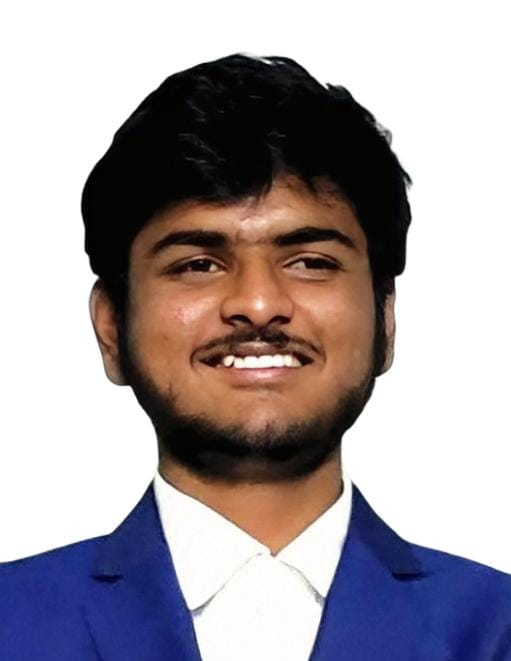
\includegraphics[width=0.2\linewidth]{images/face_photo.jpg}
\end{flushright}
\end{figure}

%---------------------------------------------------------------------------------------------------
%	META SECTION
%---------------------------------------------------------------------------------------------------

\vspace{-115pt}

\metasection{Status:}{$2^{nd}$ Year Undergraduate Student at IISER Kolkata}
\metasection{Skills:}{Python, Latex, SQL, Mathematica, Manim, Git, Data Visualization, Typst} 
\metasection{Languages:}{English (Native Proficiency), Hindi (Native Proficiency)}
\metasection{Activities:}{Lawn Tennis, Football, Coding}
\metasection{Links:}{\textcolor{sectcol}{\textbf{\href
  {https://www.linkedin.com/in/eklavya-raman-0b3595279/}
  {linkedin.com/in/eklavya-raman-0b3595279/}}}, 
  \textcolor{sectcol}{\textbf{\href
  {https://github.com/eklavya-raman}
  {github.com/eklavya-raman}}},
  
  \textcolor{sectcol}{\textbf{\href{https://eklavya-raman.vercel.app/}{eklavya-raman.vercel.app}}}}

%---------------------------------------------------------------------------------------------------
%	SUMMARAY (optional)
%---------------------------------------------------------------------------------------------------

\cvsection{Summary}

I am a second year undergraduate student at IISER Kolkata with a strong foundation in computer science and mathematics. I am passionate about computer science and mathematics and am eager to learn and potentially contribute to research in these fields. I am still exploring various areas within computer science and mathematics to find my specific interests, and I am open to opportunities that will allow me to grow my skills and knowledge.

%===================================================================================================
%	CV SECTIONS AND EVENTS (MAIN CONTENT)
%===================================================================================================

%---------------------------------------------------------------------------------------------------
%	EXPERIENCE
%---------------------------------------------------------------------------------------------------
\cvsection{Student Activities}

\cvevent{2025-2026}{Office Bearer for Lawn Tennis Club}{IISER Kolkata}
\cvdetail{Organizing and coordinating tennis events and activities for club members}
\cvdetail{Managing club resources and facilities to ensure smooth operations}

\cvevent{2024 Spring}{Latex Workshop Conductor}{IISER Kolkata}
\cvdetail{Conducted a workshop on LaTeX for scientific researchers and students}
\cvdetail{Covered topics such as document structure, formatting, mathematical typesetting, and bibliography management}

\cvevent{2024 Autumn}{IISM Participant, Lawn Tennis}{IISER Kolkata}
\cvdetail{Represented IISER Kolkata in the inter-IISER sports meet for lawn tennis}
\cvdetail{Won the silver medal in the men's team event}






%---------------------------------------------------------------------------------------------------
%	EDUCATION SECTION
%---------------------------------------------------------------------------------------------------
\cvsection{Education}

\cvevent{2024 - Current}{BS-MS Dual Degree Program}{IISER Kolkata}
\cvdetail{Pre-Majors: Physics, Mathematics and Biology}
\cvdetail{Courses: Linear Algebra I, Analysis I, Probability and Statistics I}
\cvdetail{CGPA: 7.48/10 till Semester 2}

\cvevent{2014 - 2024}{High School Diploma}{Gyan Bharati School, Saket, New Delhi}
\cvdetail{Prefect of student body}
\cvdetail{Clubs and activities: Football, Competitive Programming, Mathematics Club}
\cvdetail{Graduated with 95.4\% in CBSE Class 12 Board Exams}

\cvsection{Awards and Scholarships}

\cvevent{2024}{DST-Inspire Scholarship}{DST, Govt. of India}
\cvdetail{Awarded to top 1\% of students in the country based on performance in CBSE Class 12 Board Exams}

\cvevent{2024}{Award for Outstanding Achievements in Technical Pursuits}{Gyan Bharati School}
\cvdetail{Awarded for excellence in competitive programming and mathematics during school years}

\cvevent{2021}{Mukhya Mantri Vigyan Protsahan Pariksha (MVPP) Scholarship}{Govt. of Delhi}
\cvdetail{Awarded to top rankers in an exam conducted by the Govt. of Delhi}




\cvsection{Exam Scores}

\cvevent{2024}{IAT}{IISER Bhopal}
\cvdetail{All India Rank: 1575}

\cvevent{2024}{CBSE Class 12 Board Exams}{CBSE}
\cvdetail{Overall Percentage: 95.4\% (Physics: 91, Mathematics: 97, Computer Science: 98, Chemistry: 95, English: 96)}
\cvdetail{School Topper in CS and Chemistry}

\cvevent{2023}{IELTS}{British Council}
\cvdetail{Overall Band Score: 8.0 (Listening: 8.5, Reading: 8.5, Writing: 7.0, Speaking: 7.0)}

\cvevent{2023}{SAT}{College Board}
\cvdetail{Total Score: 1540/1600 (Math 800/800, Evidence-Based Reading and Writing 740/800)}

\cvevent{2022}{CBSE Class 10 Board Exams}{CBSE}
\cvdetail{Overall Percentage: 95.6\%}
\cvdetail{School Topper in Mathematics and Science}
%---------------------------------------------------------------------------------------------------
%	ARTIFICIAL FOOTER (fancy footer cannot exceed linewidth) 
%---------------------------------------------------------------------------------------------------

\null
\vspace*{\fill}
\hspace{-0.25\linewidth}\colorbox{bgcol}{
  \makebox[1.5\linewidth][c]{
    \mystrut \small 
    \textcolor{white}{
      \href{https://www.linkedin.com/in/eklavya-raman-0b3595279/}
      {https:/www.linkedin.com/in/eklavya-raman-0b3595279/}
    } $\cdot$ 
    \textcolor{white}{
      \href{https://github.com/john-doe}
      {https://github.com/john-doe}
    }
  }
}

%===================================================================================================
%	DOCUMENT END
%===================================================================================================
\end{document}
